% Chapter 17 -- Claim: Credit Spreads Compensate Mainly for Expected Default Losses
% Requires: amsmath, amssymb, booktabs, array, tabularx, graphicx, tcolorbox (breakable, skins), hyperref or url.
% Defines the callout box only if the preamble has not.
\providecolor{fenavy}{HTML}{1B2A6B}
\providecolor{feshade}{HTML}{F3F5FA}
\makeatletter
\@ifundefined{callout}{%
  \newtcolorbox{callout}{breakable, enhanced,
    colback=white, colframe=gray!70, boxrule=0.5pt, arc=1mm,
    borderline west={2.5pt}{0pt}{gray!70},
    left=8pt, right=8pt, top=4pt, bottom=4pt}%
}{}
\makeatother

\chapter{Claim: Credit Spreads Compensate Mainly for Expected Default Losses}
\label{ch:17}

A corporate bond pays more than a Treasury bond of similar maturity. The obvious explanation is that companies can default and the U.S. government, for practical purposes, does not. Investors demand a higher yield to cover the losses they expect when some borrowers fail to pay. On this view, the credit spread is an actuarial charge: default probability times loss given default.

The view is intuitive, it is how many investors think about credit, and it is how credit ratings are designed, since ratings rank bonds by their expected default losses. It is also testable, because a century of default data tells us how often bonds of each rating have defaulted and how much investors recovered.

This chapter tests it. The answer bears on what credit investors are paid for, why spreads rise in recessions, and why highly rated structured securities proved so dangerous in 2007--08.

By the end of the chapter you will be able to:

\begin{itemize}
  \item define credit spreads, default probabilities, recovery rates and loss given default;
  \item compute the expected-loss spread and the default rate that would justify an observed spread;
  \item explain the Merton model, in which equity is a call option on the firm's assets;
  \item distinguish real-world from risk-neutral default probabilities, and explain why the timing of defaults matters for the spread;
  \item state the claim that spreads mainly reflect expected losses, and summarize the evidence on the credit spread puzzle and the excess bond premium;
  \item judge what a credit investor is paid for, and when reaching for yield is likely to disappoint.
\end{itemize}

\section{Foundations: spreads, default and recovery}
\label{sec:17-foundations}

\textbf{Credit spread.} The yield on a corporate bond minus the yield on a Treasury of similar maturity. Moody's publishes long-run yield series for seasoned \textbf{Aaa} and \textbf{Baa} bonds, the highest and lowest investment-grade ratings, back to 1919. The \textbf{Baa--Aaa spread} compares two corporate yields and avoids some of the differences between corporate and Treasury bonds.

\textbf{Default probability (PD)} is the chance that the issuer fails to pay in a given year. Rating agencies publish historical default rates by rating. Moody's reported average annual default rates of 0.27\% for Baa issuers and essentially zero for Aaa over 1920--2006, and about 1\% for Ba, the highest speculative grade (Moody's Investors Service 2007).

\textbf{Recovery rate ($R$)} is the fraction of face value investors recover after default, measured by the bond's price shortly after default. Moody's reported an average of 38\% for senior unsecured bonds over 1982--2006. \textbf{Loss given default} is $1 - R$.

\textbf{Expected-loss spread.} A risk-neutral investor, one who cares only about expected payoffs, demands just enough extra yield to cover expected losses. For a one-year horizon with continuous compounding:
\begin{equation}
  \text{spread} = -\ln\!\left[1 - \mathrm{PD}\,(1 - R)\right] \approx \mathrm{PD}\,(1 - R)
  \label{eq:17-el}
\end{equation}
Any spread above this is compensation for something else: risk, illiquidity or taxes.

\textbf{Why spreads can exceed expected losses.}

\begin{itemize}
  \item \textbf{Risk premium.} Defaults cluster in recessions, when investors' other wealth is also falling. Risk-averse investors demand compensation for losses that arrive at bad times.
  \item \textbf{Liquidity.} Corporate bonds trade less often and at wider bid--ask spreads than Treasuries.
  \item \textbf{Taxes.} In the United States, interest on corporate bonds is subject to state income tax; interest on Treasuries is not.
\end{itemize}

\textbf{The Merton model.} Merton (1974) treated a firm's equity as a call option on its assets, with the face value of debt as the strike (Figure~\ref{fig:17-merton}). Default occurs if asset value falls below the debt at maturity. The model links credit spreads to leverage and asset volatility, and its descendants, \textbf{structural models}, are the standard tool for asking whether spreads are consistent with default risk.

\begin{figure}[htbp]
\centering
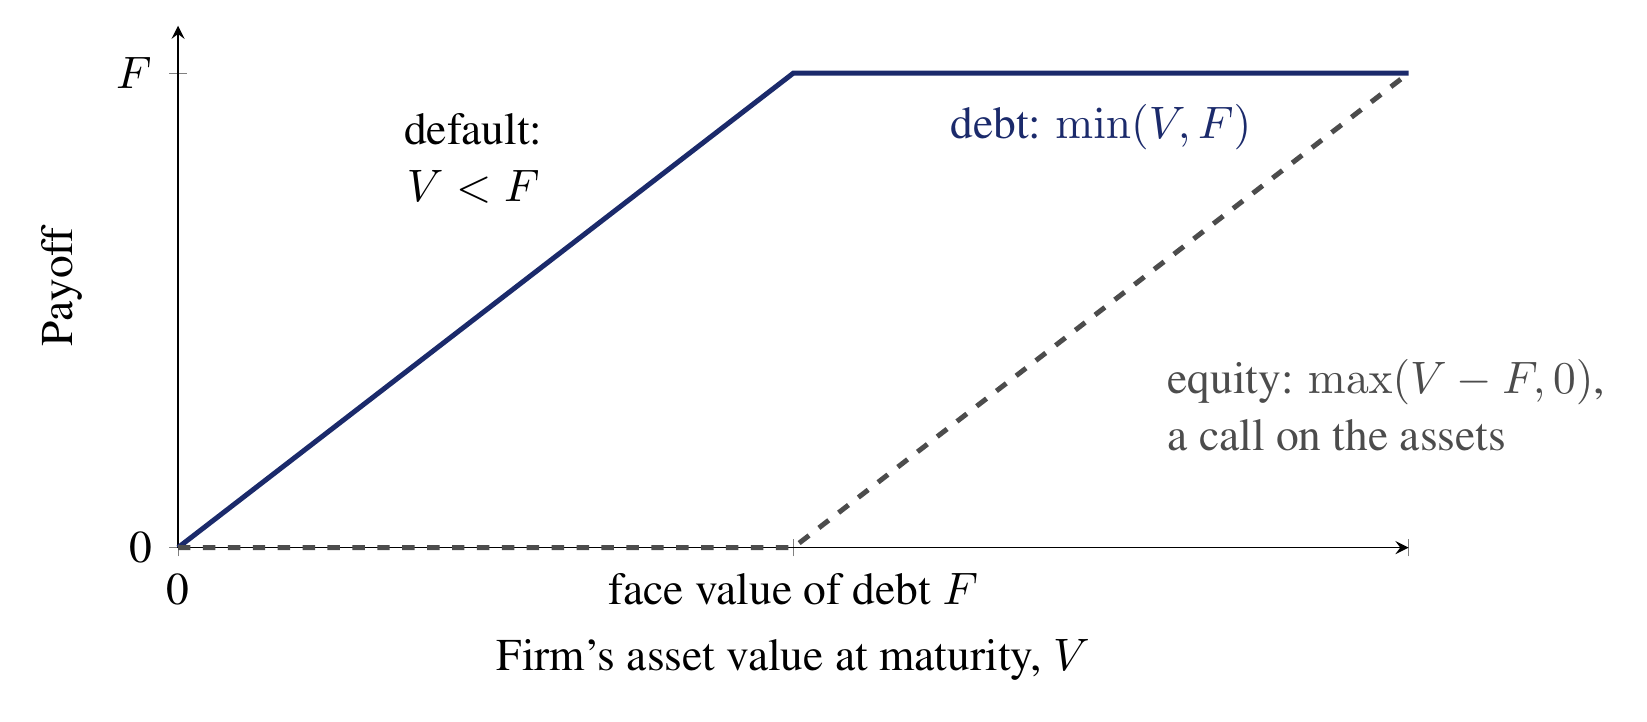
\includegraphics[width=0.85\linewidth]{images/fig17-1-merton.png}
\caption{The Merton model. At maturity, debtholders receive the firm's asset value $V$ up to the face value of debt $F$, so debt pays $\min(V, F)$. Shareholders receive what is left, $\max(V - F, 0)$, the payoff of a call option on the firm's assets. If $V < F$, the firm defaults.}
\label{fig:17-merton}
\end{figure}

\textbf{Worked example.} A 10-year Baa bond yields 6\% and a 10-year Treasury 4\%, a spread of 2\% (Figure~\ref{fig:17-decomp}).

\begin{itemize}
  \item With $\mathrm{PD} = 0.27\%$ and $R = 38\%$, the expected-loss spread is $-\ln(1 - 0.0027 \times 0.62) \approx 0.17\%$. Expected losses explain about 8\% of the spread.
  \item For expected losses to explain the whole 2\%, the annual default rate would have to be about $(1 - e^{-0.02})/0.62 \approx 3.2\%$, roughly twelve times the historical Baa average and well above the long-run average for Ba bonds.
  \item Even a pessimistic assumption, $\mathrm{PD} = 1\%$ and $R = 20\%$, explains only 0.8\% of the 2\% spread.
\end{itemize}

\begin{figure}[htbp]
\centering
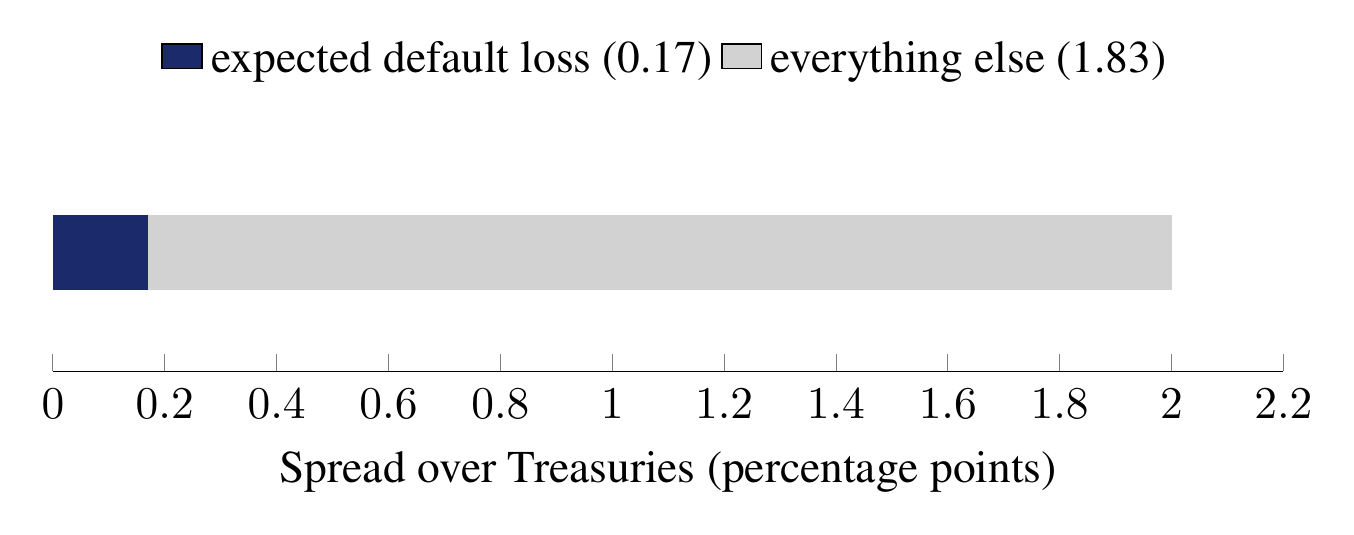
\includegraphics[width=0.85\linewidth]{images/fig17-2-spread-decomp.png}
\caption{Decomposing the worked example's 2\% Baa spread. At Moody's long-run default and recovery rates, expected default losses account for 0.17 percentage points. The remaining 1.83 points pay for something else: risk, illiquidity or taxes.}
\label{fig:17-decomp}
\end{figure}

\textbf{Further reading.} Hull, \emph{Options, Futures, and Other Derivatives} and \emph{Risk Management and Financial Institutions} (credit risk, default probabilities from bond prices, real-world versus risk-neutral probabilities, the Merton model); Fabozzi, \emph{Bond Markets, Analysis, and Strategies} (corporate bonds and credit spreads); Duffie and Singleton, \emph{Credit Risk: Pricing, Measurement, and Management}.

\section{How it works}
\label{sec:17-how}

A corporate bond's spread over a Treasury can be split into four pieces:

\begin{center}
\small
\begin{tabularx}{0.9\linewidth}{@{}>{\raggedright\arraybackslash}p{0.2\linewidth}>{\raggedright\arraybackslash}X>{\raggedright\arraybackslash}X@{}}
\toprule
Component & What it pays for & How to measure it \\
\midrule
Expected default loss & The average loss from defaults & Historical default rates $\times$ loss given default \\
Default risk premium & Bearing default losses that cluster in bad times & Residual after expected loss; structural models \\
Liquidity premium & Costs and delays of trading corporate bonds & Bid--ask spreads, trading volume, bond-specific measures \\
Tax premium & State taxes on corporate interest & Tax rates applied to the yield \\
\bottomrule
\end{tabularx}
\end{center}

The claim is that the first component dominates. The test has two steps. First, estimate expected losses from historical default and recovery data and compare them with observed spreads. If they explain most of the spread, the claim survives. Second, examine the residual. If it is small and stable, it might be liquidity or measurement error. If it is large, rises in recessions and forecasts economic activity, it behaves like a risk premium.

\textbf{Real-world and risk-neutral probabilities.} Bond prices imply a \textbf{risk-neutral} default probability: the default rate that would justify the spread for an investor who does not care about risk. Historical data give \textbf{real-world} default probabilities. The gap between the two measures how much investors charge for bearing default risk. Hull's textbooks show this gap is large for investment-grade bonds and smaller, relative to the spread, for junk bonds.

\textbf{Why the timing of defaults matters.} Two bonds with the same expected loss can deserve very different spreads. A bond whose defaults occur randomly over the cycle adds little risk to a diversified portfolio. A bond whose defaults all arrive in recessions, when stocks are falling and jobs are at risk, is much less attractive and should pay more. Investment-grade defaults are rare in normal times and concentrated in severe downturns, which is exactly the pattern that should command a large premium.

\section{The claim}
\label{sec:17-claim}

\begin{callout}
\textbf{Claim.} The yield spread of corporate bonds over Treasuries mostly reflects the losses investors expect from default. Under reasonable assumptions for default rates and recoveries, expected losses account for most of the average spread.
\end{callout}

To test it we need to be precise on three points.

\begin{itemize}
  \item \textbf{Mostly.} We take ``mostly'' to mean more than half of the average spread for investment-grade bonds. The claim could hold for junk bonds and fail for investment grade, or the reverse.
  \item \textbf{Reasonable assumptions.} Default and recovery rates vary over time and by measurement. The test uses long-run averages from rating agencies and checks how far they would have to be stretched to rescue the claim.
  \item \textbf{What would count against it.} The claim fails if expected losses explain less than half of investment-grade spreads under any plausible assumptions, and if the remainder behaves like compensation for risk: rising in recessions and forecasting weaker economic activity.
\end{itemize}

\section{The original evidence}
\label{sec:17-evidence}

\textbf{Elton, Gruber, Agrawal and Mann (2001).} Using corporate bond prices and historical default and recovery rates, they found that expected default losses accounted for only a small part of the spread between corporate and Treasury yields. State taxes, which apply to corporate interest but not to Treasury interest, explained a large part. The rest moved with the risk factors that explain stock returns, evidence of a risk premium.

\textbf{Collin-Dufresne, Goldstein and Martin (2001).} If spreads reflect default risk, changes in spreads should be explained by changes in the variables that drive default in structural models: leverage, asset volatility, interest rates. These explained only about a quarter of the variation in spread changes. Most of the rest was driven by a single common factor across bonds, unrelated to firm-specific default risk.

\textbf{Huang and Huang (2012).} They calibrated a wide range of structural models to historical default losses and equity risk premia and asked how much of observed spreads the models could explain. For investment-grade bonds, credit risk accounted for only a small share of spreads, and an even smaller share at short maturities. For high-yield bonds, it accounted for much more. This gap became known as the \textbf{credit spread puzzle}.

\textbf{Gilchrist and Zakraj\v{s}ek (2012).} They split corporate spreads into a component explained by expected default, estimated firm by firm, and a residual they called the \textbf{excess bond premium}. The excess bond premium, not the default component, carried most of the information about future economic activity. A rise in it predicted lower output and employment, consistent with a measure of investors' risk appetite and of the health of financial intermediaries.

Some later work narrows the puzzle by modelling default risk that varies with the business cycle. None restores expected losses as the main component of investment-grade spreads.

\section{Replication lab: a century of corporate spreads}
\label{sec:17-lab}

\begin{callout}
\textbf{Lab 17 at a glance.} \emph{Claim on trial:} credit spreads mainly reflect expected default losses. \emph{Data:} free monthly data from FRED: Moody's seasoned Aaa and Baa yields from 1919, the 10-year Treasury yield from 1953, the NBER recession indicator and industrial production. The Gilchrist--Zakraj\v{s}ek excess bond premium, published by the Federal Reserve, can be added. \emph{Code:} runs as a script (\texttt{python lab17.py}) or as a notebook with a prediction prompt before each step.
\end{callout}

\textbf{Part A, spreads.} The Baa--Aaa spread since 1919 and the Baa--Treasury and Aaa--Treasury spreads since 1953: averages, decade averages, and averages in recessions and expansions (Figure 17.3).

\textbf{Part B, decomposition.} The expected-loss spread from adjustable assumptions, by default 0.27\% a year for Baa and zero for Aaa with 38\% recovery, Moody's long-run averages. The lab reports the share of each average spread that expected loss explains, and the default rate that would be needed for expected loss to explain the whole spread at each date (Figures 17.4 and 17.5).

\textbf{Part C, the residual as a risk premium.} Regressions of industrial production growth over the next 12 months on each spread, and on the excess bond premium if supplied; growth by spread quintile; and the average path of the Baa--Aaa spread around the start of recessions (Figure 17.6).

\textbf{Part D, stress tests.} The share of the Baa--Treasury spread explained over a grid of default rates from 0.1\% to 2\% and recoveries from 20\% to 60\% (Figure 17.7), spread peaks in six crises, and subperiod averages.

Three measurement issues affect the decomposition, and they work in different directions.

\begin{itemize}
  \item \textbf{Maturity.} Moody's yields are on long bonds, typically 20 years or more, while the Treasury benchmark is 10 years. When the Treasury curve slopes up, this widens the Baa--Treasury spread for reasons unrelated to credit. The Baa--Aaa spread avoids the problem.
  \item \textbf{Taxes.} State taxes on corporate interest widen corporate--Treasury spreads, but not the Baa--Aaa spread.
  \item \textbf{Default timing.} Annual average default rates understate losses in the worst decades, such as the 1930s. Part D's grid includes default rates several times the average.
\end{itemize}

\textbf{What the simulated run shows.} The simulation builds the Baa--Aaa spread from a fixed expected loss of 0.15\% plus a premium that jumps in recessions. The lab recovers it: expected loss explains about a quarter of the Baa--Aaa spread, the spread is higher in recessions, and a high spread forecasts weaker output growth. These results confirm that the code works. They say nothing about real markets. Run the lab on the real data to reach your own verdict.

\section{Stress tests}
\label{sec:17-stress}

\textbf{Default assumptions.} The obvious defence of the claim is that historical averages understate future defaults. Part D's grid shows how far the assumptions must be stretched. With the 1920--2006 Baa average of 0.27\%, expected loss is a small fraction of a spread of one to two percentage points. To explain most of it, Baa bonds would need to default at well over 1\% a year with low recoveries, every year, which is the long-run experience of speculative-grade Ba bonds, not investment-grade Baa.

\textbf{The Great Depression.} The 1930s are the worst case for investment-grade defaults in the Moody's data. A default rate several times the long-run Baa average in those years would raise the expected-loss share sharply for that decade. Even then, the claim must explain the spread in the many decades with almost no Baa defaults.

\textbf{Crises.} Spreads peak in crises: the early 1930s, 1974--75, 1980--82, 2008--09 and March 2020. If spreads were expected losses, the peaks would forecast correspondingly large defaults. In 2008--09 and 2020, investment-grade defaults rose but remained far below what the peak spreads would have required. Spreads widened mainly because investors demanded more to hold risk and because dealers and funds withdrew from the market.

\textbf{Rating categories.} For high-yield bonds, expected losses are a much larger share of the spread (Huang and Huang 2012). The claim may work for junk bonds and fail for investment grade. Moody's yield series cover only Aaa and Baa, so this lab cannot test it directly; Exercise 1 extends the decomposition using published default rates for lower ratings.

\textbf{Liquidity.} Part of the residual is compensation for illiquidity, and it rises in crises when trading dries up. Separating liquidity from risk is difficult because both rise together in bad times. The Gilchrist--Zakraj\v{s}ek excess bond premium, which strips out firm-level default risk, is a useful check: if it forecasts output as well as the raw spread, the forecasting power does not come from expected defaults.

\section{Verdict}
\label{sec:17-verdict}

\begin{callout}
\textbf{Verdict: fails} (as of October 2026) for investment-grade bonds. Under historical default and recovery rates, expected default losses explain only a minority of investment-grade spreads, and the remainder behaves like a risk premium that rises in bad times and forecasts weaker economic activity. For high-yield bonds the claim fits better, since expected losses are a much larger share of their spreads.
\end{callout}

What fails:

\begin{itemize}
  \item \textbf{Expected losses are too small.} With Moody's long-run Baa default rate of 0.27\% and 38\% recovery, expected loss is under 0.2 percentage points a year, a small fraction of typical Baa spreads. Rescuing the claim requires default rates several times higher, sustained over decades.
  \item \textbf{Spreads move for other reasons.} Changes in default-risk variables explain only a quarter of spread changes (Collin-Dufresne, Goldstein and Martin 2001), and a common factor drives much of the rest.
  \item \textbf{The residual is a risk premium.} It rises in recessions, peaks in crises and forecasts weaker output, which is how compensation for bearing risk in bad times should behave (Gilchrist and Zakraj\v{s}ek 2012).
\end{itemize}

What survives:

\begin{itemize}
  \item \textbf{Expected losses matter at the margin.} Lower-rated bonds have higher spreads, and expected losses rise with them. Ratings rank spreads correctly even though they do not explain their level.
  \item \textbf{The claim fits junk bonds better.} For speculative-grade debt, expected losses are a large share of the spread.
\end{itemize}

The verdict would move to \emph{weakens} if a measure of liquidity explained most of the residual and that liquidity premium did not vary with economic conditions. The evidence so far points the other way: the residual and liquidity both rise in bad times.

\section{What investors can use}
\label{sec:17-investors}

\textbf{Credit is compensation for recession risk.} An investor in investment-grade bonds earns a spread well above expected default losses. That is good news on average, but it is pay for a specific risk: losses and price declines that arrive together with stock-market losses and recessions. Credit is not a substitute for Treasuries in a portfolio meant to hedge equity risk.

\textbf{The limits of reaching for yield.} In low-rate periods, investors move into lower-rated or longer-maturity credit to earn more. The extra yield is real, but it is paid for bearing more of the same recession risk. A portfolio that has quietly accumulated credit exposure will behave like an equity portfolio in a downturn.

\textbf{Ratings measure expected loss, not timing.} A rating ranks bonds by how likely they are to default and how much investors will lose, on average. It says nothing about whether those losses will arrive in a recession, which is what determines the risk premium.

\textbf{Questions to ask a credit manager:}

\begin{itemize}
  \item What share of the portfolio's yield above Treasuries would be lost in a recession with default rates like those of 2009?
  \item How correlated are the portfolio's returns with stocks in bad months?
  \item How liquid are the holdings in a crisis, and what would it cost to sell them?
  \item For structured holdings, how do losses depend on correlations between the underlying loans?
\end{itemize}

\begin{callout}
\textbf{What Failed: highly rated structured credit before 2008.} By 2007, according to Fitch, roughly 60\% of all global structured products carried AAA ratings, compared with less than 1\% of corporate issues (Coval, Jurek and Stafford 2009). Pooling mortgages and other loans and slicing them into \textbf{tranches}, claims with different priority on the pool's losses, allowed issuers to create large quantities of senior securities whose expected default losses, as estimated by rating models, were as low as those of the safest corporate bonds. They were priced accordingly, with spreads similar to other AAA debt.

The mistake was the claim this chapter tests: that a spread need only compensate for expected losses. Senior tranches lose money only when many underlying loans default together, which happens in a severe recession. Their losses are therefore concentrated in exactly the worst states of the world, and they deserved much larger risk premiums than corporate bonds with the same expected loss. In 2007, Moody's downgraded 31\% of the asset-backed CDO tranches it rated, including 14\% of those initially rated AAA, and many more were downgraded in 2008. Investors who had treated rating-based expected losses as the whole story discovered that the timing of losses matters as much as their average.
\end{callout}

\section{Open questions}
\label{sec:17-open}

\begin{itemize}
  \item \textbf{How much of the residual is liquidity rather than risk?} Both rise in bad times. Better measures of bond-level liquidity, and the growth of bond ETFs, offer new ways to separate them.
  \item \textbf{Has the investor base changed spreads?} Insurance companies, bond funds and ETFs hold most corporate bonds. Do their constraints, such as capital rules tied to ratings or redemption pressure, create premiums unrelated to default?
  \item \textbf{What did central-bank purchases do?} In 2020 the Federal Reserve announced purchases of corporate bonds, and spreads fell sharply. How much of the premium is the price of intermediaries' balance-sheet capacity?
  \item \textbf{Do structural models need fixing or replacing?} Models with time-varying risk and macroeconomic default risk narrow the credit spread puzzle. Do they fit the cross-section of spreads by rating and maturity as well as the average?
\end{itemize}

\section*{Exercises}
\addcontentsline{toc}{section}{Exercises}

\subsection*{Conceptual (all readers)}

\begin{enumerate}
  \item Using Moody's long-run average annual default rates (Ba about 1.1\%, B about 3.5\%) and 38\% recovery, compute the expected-loss spread for Ba and B bonds. If typical spreads are 3\% and 5\%, what share is expected loss? Compare with the Baa result.
  \item A 5-year Baa bond yields 5.5\% and the 5-year Treasury 4\%. What annual default rate, with 40\% recovery, would make expected losses equal the spread? What does this say about the risk-neutral and real-world default probabilities?
  \item Explain in words why a bond whose defaults all occur in recessions should pay a higher spread than one with the same expected loss whose defaults occur at random times.
\end{enumerate}

\subsection*{Lab extensions (technical readers)}

\begin{enumerate}
  \setcounter{enumi}{3}
  \item Part B: with the default assumptions, what share of the Baa--Treasury and Baa--Aaa spreads does expected loss explain? Why might the two shares differ?
  \item Part B: plot the break-even default rate. In which months was it lowest? Was it ever below the historical Baa default rate?
  \item Part C: does the Baa--Aaa spread forecast industrial production growth? If you have the excess bond premium, does it forecast better?
  \item Part D: find the default and recovery assumptions under which expected loss explains 75\% of the average Baa--Treasury spread. Are they plausible for investment-grade bonds?
  \item Subtract an estimate of the state tax effect (for example, a 4\% tax rate applied to the corporate yield) and recompute the residual. How much does it shrink?
  \item A pension fund wants to raise its yield by moving from Treasuries to Baa corporate bonds. Using this chapter's evidence, explain what the fund will be paid for and when it is likely to regret the move.
\end{enumerate}

\section*{References}
\addcontentsline{toc}{section}{References}

\begin{itemize}
  \item Collin-Dufresne, P., Goldstein, R. S. and Martin, J. S. (2001). The Determinants of Credit Spread Changes. \emph{Journal of Finance} 56(6): 2177--2207.
  \item Coval, J., Jurek, J. and Stafford, E. (2009). The Economics of Structured Finance. \emph{Journal of Economic Perspectives} 23(1): 3--25.
  \item Elton, E. J., Gruber, M. J., Agrawal, D. and Mann, C. (2001). Explaining the Rate Spread on Corporate Bonds. \emph{Journal of Finance} 56(1): 247--277.
  \item Gilchrist, S. and Zakraj\v{s}ek, E. (2012). Credit Spreads and Business Cycle Fluctuations. \emph{American Economic Review} 102(4): 1692--1720.
  \item Huang, J.-Z. and Huang, M. (2012). How Much of the Corporate-Treasury Yield Spread Is Due to Credit Risk? \emph{Review of Asset Pricing Studies} 2(2): 153--202.
  \item Merton, R. C. (1974). On the Pricing of Corporate Debt: The Risk Structure of Interest Rates. \emph{Journal of Finance} 29(2): 449--470.
  \item Moody's Investors Service (2007). \emph{Corporate Default and Recovery Rates, 1920--2006}. New York: Moody's.
\end{itemize}

\textbf{Data:} FRED, Federal Reserve Bank of St.\ Louis: Moody's Seasoned Aaa Corporate Bond Yield [AAA], Moody's Seasoned Baa Corporate Bond Yield [BAA], 10-Year Treasury Constant Maturity Rate [GS10], NBER Recession Indicator [USREC], Industrial Production [INDPRO]. Optional: Federal Reserve Board, Gilchrist--Zakraj\v{s}ek excess bond premium.
